\documentclass[]{scrartcl}
\usepackage{graphicx}
\usepackage{color}
\usepackage{hyperref}
\usepackage{calc} 
\usepackage{enumitem}
\newcommand{\source}[1]{\vspace{-3pt} \caption*{ Source: {#1}} }
%\pagestyle{headings}

% customize dictum format:
\usepackage[T1]{fontenc}
\setkomafont{dictumtext}{\itshape\small}
\setkomafont{dictumauthor}{\normalfont}
\renewcommand*\dictumwidth{\linewidth}
\renewcommand*\dictumauthorformat[1]{--- #1}
\renewcommand*\dictumrule{}
\newcommand{\todo}[1]{\textcolor{red}{TODO: #1}\PackageWarning{TODO:}{#1!}}

\begin{document}

\title{
	\includegraphics*[width=0.63\textwidth]{images/yale_logo.png}\\
	\vspace{24pt}
	ENGL 300:\\Introduction to Theory of Literature}
\subtitle{Lecture Spring, 2009\\
          Paul H. Fry\\
          William Lampson Professor of English \\ 
          Yale University}
\author{Lennard Wolf\\
        \href{mailto:lennard.wolf@student.hu-berlin.de}{lennard.wolf@student.hu-berlin.de}}
\maketitle
\begin{abstract}

This is a survey of the main trends in twentieth-century literary theory. Lectures will provide background for the readings and explicate them where appropriate, while attempting to develop a coherent overall context that incorporates philosophical and social perspectives on the recurrent questions: what is literature, how is it produced, how can it be understood, and what is its purpose?

\end{abstract}
\newpage

\tableofcontents

\listoffigures
\newpage


\section{Introduction I}


\subsection{Description Text}
\dictum[William Wordsworth, \textit{The Friend, 1805}]{%
Bliss was it in that dawn to be alive}
\vspace{15pt}

In this first lecture, Professor Paul Fry explores the course's title in three parts. The relationship between theory and philosophy, the question of what literature is and does, and what constitutes an introduction are interrogated. The professor then situates the emergence of literary theory in the history of modern criticism and, through an analysis of major thinkers such as Marx, Nietzsche, and Freud, provides antecedents for twentieth-century theoretical developments.

\subsection{Content}
\dictum[Georg Wilhelm Friedrich Hegel, \textit{Die Vernunft in der Geschichte}]{%
Was der Geist will, ist, seinen eigenen Begriff erreichen (den Ort an dem er theoretisch und praktisch in Harmonie mit dem Ganzen steht); aber er selbst verdeckt sich denselben, ist stolz und voll Genu\ss~in dieser Entfremdung seiner selbst.}
\vspace{15pt}

Literature can not really be defined clearly, as exceptions to the rule always persist. However defining it helps us deal with complexity, and to understand what literature is, is in part goal of this lecture. \emph{Theory} has the goal of analyzing the text to for example understand its meaning and can thus be put to practice using certain methodologies. Questions raised by Literary Theory can be \emph{"What is a reader/an author?"} etc.

Scepticism has its roots in \emph{Modernity} (generation of Descartes, Shakespeare, and Cervantes), with thinkers starting to question common assumptions (like Descartes in his \emph{Meditations}: \emph{"Well, might I not be crazy?"}). In 1796, Kant further questioned the relationship of our knowledge of the world with its reality (\emph{"We cannot know the thing in itself."}). Then, in his 1807 book \emph{The Phenomenology of Mind}, Hegel says that these developments in thought have formed a sort of \emph{Entfremdung}, through which we are driven away from our goal to know ourselves.

Modern skepticism has three central figures: Marx, Nietzsche, and Freud. Their core thoughts which are relevant here are the following:

\begin{description}[leftmargin=!,labelwidth=\widthof{\bfseries Nietzsche}]
  \item[Marx] In \emph{Kapital}, M. talks about \emph{commodity fetishism}, through which we assign "objective" value to commodities, such as human labor. He then compares commodity fetishism to the belief in God, stating that both are determined by social, historical, and economic factors, and are both part of \textbf{ideology}, which the ideologically thinking person can not escape.
  \item[Nietzsche] For N., the underpinnings of consciousness which make the operations of consciousness inauthentic are the nature of \textbf{language} itself. "\emph{What then is truth? A mobile army of metaphors, metonymies, anthropomorphisms--in short, a sum of human relations which became poetically and rhetorically intensified,}" etc., etc., etc., "\emph{and are now no longer of account as coins but are debased.}". However, N. believed that once there was a moment in language time, were that was not the case and only truth was said.
  \item[Freud] In \emph{The Psychopathology of Everyday Life}, F. says that after all, we have absolutely no objective evidence that the unconscious exists. If I could see the unconscious, it'd be conscious. The unconscious is something that we have to infer from the way consciousness operates. We've got to figure out somehow how it is that consciousness is never completely uninhibited, never completely does and says what it wants to say. So the spin on consciousness for Freud is the \textbf{unconscious}.
  
\end{description}

Now, we do not only have no knowledge of ourselves, but also none about the objects around us and their relationship with us. This has perplexed many people, and so many large, angry volumes were written against such skepticism and the literary theory that it had sparked.

\subsection{New Words}

\begin{description}[leftmargin=!,labelwidth=\widthof{\bfseries Cartesian Revolution}]
  \item[Literature] Literature can not really be defined clearly, as exceptions to the rule always persist. Thus definitions of literature can always only exist in a certain context.
  \item[Hermeneutics] The science of interpreting and understanding of human symbols, usually in the form of text.
  \item[Literary Theory] In contrast to \emph{Literary Criticism}, Literary Theory is not concerned with opinionating and defining the value of a text, but rather with systematically analyzing and dwelling on it, while considering history, philosophy, and other fields which are relevant to the interpretation of meaning. Today, it is often referred to as \emph{Theory} in the academic world.
  \item[Modernity] (Not to be confused with \emph{Modernism}, which is a more nuanced cultural movement in late Modernity) Coined by Baudelaire in his essay \emph{The Painter of Modern Life}. Historical period (1453 - 1989), in which first through art and later all other sciences tradition is more and more questioned and rejected. Individualism, freedom, and formal equality are key values.
  \item[Cartesian Revolution] Begin of rationalist thought after Descartes
  \item[Verfremdung] ??
\end{description}

\section{Introduction II}

\dictum[Immanuel Kant, \textit{Reflexionen}]{%
Er ist ein Egoist der Wissenschaft, und es ist ihm noch ein Auge n\"otig, welches macht, dass er seinen Gegenstand noch aus dem Gesichtspunkte anderer Menschen ansieht...}
\vspace{15pt}

\subsection{Description Text}
In this second introductory lecture, Professor Paul Fry explores the interrelation of skepticism and determinism. The nature of discourse and the related issue of \emph{discursivity} is read through two modern works, Anton Chekov's \emph{Cherry Orchard} and Henry James' \emph{The Ambassadors}. Exemplary critical focus on literary authority is located in Michel Foucault's \emph{What Is an Author} and Roland Barthes' \emph{The Death of the Author}, both of which are read with an emphasis on their historical contexts. Objections to the approach and conclusions of the two theorists are examined, particularly in light of the rise of cultural studies.

\subsection{Content}


\subsection{New Words}

\begin{description}[leftmargin=!,labelwidth=\widthof{\bfseries Cartesian Revolution}]
  \item[Literature] asdf
\end{description}


\newpage
\section{Meta}
\subsection{The Professor}
Prof. Paul H. Fry (see Figure \ref{fig:paul_fry}) received his B.A. from University of California, Berkeley in 1966 and earned his Ph.D. in 1973 from Harvard University, where he had writ7ten his dissertation \emph{"Byron’s Myth of the Self"}. He has taught at Yale University since 1971, became Assistant Professor of English in 1973, Associate Professor of English in 1979, Professor of English in 1985 and William Lampson Professor of English in 1993.

\begin{figure}[]
	\centering
	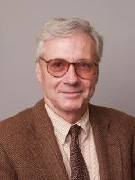
\includegraphics[width=0.32\textwidth]{images/paul_fry.jpg}
	\caption{Prof. Paul Fry. Source: \url{https://www.library.yale.edu/judaica/site/conferences/Amichai/Speaker\%20pics/roundtable/Fry_1051.jpg}}
	\label{fig:paul_fry}
\end{figure}

\subsection{Texts}

Richter, David, ed. The Critical Tradition, 3rd ed. (Bedford-St. Martin's, 2006)


\end{document}
